\section{Operationally Accessible Entanglement Entropy}

The quantum entanglement present between the constituents of a system can be quantified via von Neumann and R\'enyi entanglement entropies. These measures have been shown to be sensitive to phase transitions in physical models, which is one of the reasons for the study of quantum entanglement. But, what about using entanglement as a resource for, let's say, quantum computing? For this purpose, the entanglement entropies have to be redefined such that they obey constraints imposed by performing a measurement on a system. These physical constraints imposed on the quantum systems that can be prepared are known as superselection rules (SSR) and can be based off particle number or spin conservation, for example. The amount of entanglement that is actually accessible as a resource is then subject to these SSR's.

In this chapter, the accessible entanglement entropy is presented. In the first section, a review of the von Neumann and R\'enyi entanglement entropies is given. In the second, analytical values for the spatial entanglement entropies are derived at various regimes of the $t-V$ model. Finally, numerical results obtained via exact diagonalization are presented.

\subsection{The \ren Entanglement Entropy}
\label{sec:accEntanglementIntro}

The amount of entanglement that exists between some partition $A$ and its compliment $B$ of a quantum many-body system in pure state $\ket{\Psi}$ can be quantified via the R\'{e}nyi entanglement entropy which depends on an index $\alpha$:
%
\begin{equation}
S_{\alpha} (\rho_A) = \frac{1}{1-\alpha}\ln \Tr\, \rho_A^{\alpha}
\label{eq:S_alpha}
\end{equation}
%
where $\rho_{A}$ is the reduced density matrix of partition $A$ obtained by
tracing out all degrees of freedom in $B$ from the full density matrix:
%
\begin{equation}
\rho_{A} = \Tr_{B}\, \rho = \Tr_{B} \ket{\Psi}\bra{\Psi}\,.
\end{equation}
%
The \ren entropy is a monotonically decreasing function of $\alpha$ for $\alpha
> 1$ and is bounded from above by the von Neumann entropy, $S_1(\rho_A) = -\Tr \rho_A \ln \rho_A$.

For a quantum many-body system subject to physical laws conserving some quantity (particle number, charge, spin, etc.), the set of local operations on the state $\ket{\Psi}$ are limited to those that don't violate the corresponding global superselection rule.  For the remainder of this paper, we will focus on our discussion on the case of fixed total $N$ and thus we are restricted to only those operators which locally preserve the particle number in $A$.  The effect this has on the amount of entanglement that can be transferred to a qubit register is apparent from the simple example (adapted from Ref.~\cite{Wiseman:2003vn} of one particle confined to two spatial modes $A$ and $B$ corresponding to site occupations.  Then, for the state $\ket{\Psi} = \left(\ket{1}_A \otimes \ket{0}_{B} + \ket{0}_A \otimes \ket{1}_{B} \right)/\sqrt{2}$, Eq.~\eqref{eq:S_alpha} gives that $S_1 = \ln 2$. However, this entanglement cannot be transferred to a register prepared in initial state $\ket{0}_R$ via a $\texttt{SWAP}$ gate. In quantum circuits, a $\texttt{SWAP}$ in Hilbert Space $A$, will take the state of the $A$ subregion of a resource, and swap it with the state of the $A$ subregion of a register. Let $\ket{\Psi}$ be the resource state and $\ket{0}_R$ the register, then acting with a $\texttt{SWAP}$ gate gives:
%
\begin{align*}
    & \texttt{SWAP} \ket{0}_R\otimes\left(\ket{1}_A \otimes
    \ket{0}_{B} + \ket{0}_A \otimes \ket{1}_{B} \right)/\sqrt{2} \\
    &= \frac{1}{\sqrt{2}}\left( \ket{0}_R \otimes \ket{0}_A \otimes
        \ket{1}_{B} + \ket{1}_R \otimes \ket{0}_A \otimes
    \ket{0}_{B} \right)
    % &= \frac{1}{\sqrt{2}}\ket{0}_R \otimes \ket{0}_A \otimes
    %     \ket{1}_{B}
\end{align*}
The last term is not physically allowed due to the restriction that the number of particles in the system is fixed to be 1. The post-swap result remains in a product state and the amount of transferable entanglement is identically zero. The $\texttt{SWAP}$ gate in the example above takes the register modes and exchanges them with the modes in subsystem $A$ of the resource:
%
\begin{equation}
\texttt{SWAP} \ket{\phi}_R \otimes \ket{\psi}_A = \ket{\psi}_R \otimes \ket{\phi}_A
\end{equation}
%
The $\texttt{SWAP}$ can be defined such that it exchanges resource modes with modes in $B$ instead. Formally, this gate is a product of three controlled-not ($\texttt{CNOT}$) gates:
%
\begin{equation}
\texttt{SWAP} \ket{\phi}_R \otimes \ket{\psi}_A = \texttt{CNOT}_{R,A} \texttt{CNOT}_{A,R} \texttt{CNOT}_{R,A} \ket{\phi}_R \otimes \ket{\psi}_A
\end{equation}
%
where the subscript left to the comma denotes the control mode and the one to the right of the comma, the target. The $\texttt{CNOT}$ acts on qubit modes. That is, each of the modes will be either one of two values, call them 1 and 0. If the control qubit is equal to 1, then the value of the target is 'flipped' to the other possible value. If the control qubit is 0, the target is left unchanged.

\subsection{von Neumann Accessible Entanglement: $\alpha = 1$}
% ---------------------------------------------------------------------------

Thus, Eq.~\eqref{eq:S_alpha}, which includes the effects of non-local number fluctuations between $A$ and $B$, overcounts the amount of entanglement that can be accessed from the system.  To quantify the physical reduction, Wiseman and Vaccaro \cite{Wiseman:2003jx} suggested that for the case of $\alpha = 1$ a more appropriate measure should weight contributions to the entanglement coming from each superselection sector corresponding to the number of particles $n$ in $A$:
%
\begin{equation}
    S_1^{\rm{acc}}(\rho_A)=\sum_{n=0}^{N} P_n S_1(\rho_{A_n})
\label{eq:S1acc}.
\end{equation}
%
Here $\rho_{A_{n}}$ is defined to be the reduced density matrix of $A$, projected onto the subspace of fixed local particle number $n$ 
%
\begin{equation}
    \rho_{A_n} = \frac{1}{P_n}{\mathcal{P}}_{A_n} \rho_{A} {\mathcal{P}}_{A_n}
\label{eq:rhoAn}
\end{equation}
%
accomplished via a projection operator ${\mathcal{P}}_{A_n}$ where
${\mathcal{P}}_{A_n} \ket{\Psi} = \ket{n}_A\otimes\ket{N-n}_{B}$.  
$P_n$ is the probability of measuring $n$ particles in $A$:
%
\begin{equation}
    P_n = \mathrm{Tr}\, {\mathcal{P}}_{A_n} \rho_A{\mathcal{P}}_{A_n}
    = \expval{{\mathcal{P}}_{A_n}}{\Psi}.
    \label{eq:Pn}
\end{equation}
%
As the projection constitutes a local operation which can only decrease
entanglement,  it is clear that $S_1^{\rm acc}(\rho_A) \le S_1(\rho_A)$. 
Moreover, the difference 
%
\begin{equation}
    \Delta S_1 (\rho_A) \equiv S_1(\rho_A) - S_1^{\rm acc}(\rho_A)
    \label{eq:DeltaS1}
\end{equation}
%
can be determined  by noting that the superselection rule guarantees that $[\rho_A,\hat{n}]=0$ where $\hat{n}$ is the number operator acting in partition $A$. Thus $\rho_A$ is block-diagonal in $n$ and it can be shown \cite{Klich:2008se} that 
%
\begin{equation}
    \Delta S_1 (\rho_A) =  H_1(\{P_n\})
\label{eq:DS1H1}
\end{equation}
%
where
%
\begin{equation}
    H_1(\{P_n\}) = -\sum_{n=0}^N P_n \ln P_n.
\label{eq:H1}
\end{equation}
%
is the Shannon entropy of the number probability distribution.  It is instructive to consider \Eqref{eq:DS1H1} for the special case of a discrete Gaussian distribution, $P_n \propto e^{-(n-\expval{n})^2/2\sigma^2}$ where $H_1 = \ln\left(2\pi e \sigma^2 + \tfrac{1}{12}\right)$ depends only on the variance of $P_n$
%
\begin{equation}
    \sigma^2 \equiv \expval{n^2}-\expval{n}^2 = \sum_{n=0}^N n^2 P_n  - \left(\sum_{n=0}^N n P_n\right)^2\,.
\label{eq:sigma2}
\end{equation}
%
Thus, when the number fluctuations are Gaussian, the von Neumann accessible entanglement is completely determined by the variance.

% ---------------------------------------------------------------------------
\subsection{\ren Accessible Entanglement: $\alpha \ne 1$}
% ---------------------------------------------------------------------------

Computing the accessible entanglement for a many-body system is a difficult task for $\alpha=1$, as full state tomography is required to reconstruct the density matrix $\rho$. However, for integer values with $\alpha > 1$ a replica trick can be used to recast $\mathrm{Tr} \rho_A^\alpha$ as the expectation value of some local operator \cite{Calabrese:2004hl}. This advance has led to a boon of new entanglement results using both computational \cite{Hastings:2010dc, Humeniuk:2012cq, McMinis:2013dp, Herdman:2014ey, Drut:2015fs} and experimental \cite{Daley:2012bd, Islam:2015cm, Kaufman:2016ep, Pichler:2016ec, Linke:2017tf, Lukin:2018wg} methods.  Motivated by this progress, \cite{Barghathi:2018oe} generalized the accessible entanglement to the case of \ren entropies with $\alpha \ne 1$ and found that:
%
\begin{equation}
S_{\alpha}^{{\rm acc}} (\rho_A) = \frac{\alpha}{1-\alpha}\ln\left[ \sum_{n} P_n \mathrm{e}^{\frac{1-\alpha}{\alpha} S_{\alpha}(\rho_{A_n})}\right]
\label{eq:S_alpha_acc}
\end{equation} 
%
% which reproduces Eq.~\eqref{eq:S1acc} in the limit $\alpha \to 1$. While not physically transparent in this form, the modification from the $\alpha=1$ case results from replacing the geometric mean in Eq.~\eqref{eq:S1acc} with a general power mean whose form is constrained by the physical requirement that $0 \le \Delta S_\alpha \le \ln (N+1)$.  It can also be interpreted as the quantum generalization of the conditional classical \ren entropy \cite{Cachin97entropymeasures,GolshaniPashaYari:2009,Hayashi:2011,SKORIC:2011el,FehrBerens2014} subject to physical constraints \cite{Barghathi:2018oe}. The arguments leading to Eq.~\eqref{eq:DS1H1} can also be generalized leading to 
which reproduces Eq.~\eqref{eq:S1acc} in the limit $\alpha \to 1$. While not physically transparent in this form, the modification from the $\alpha=1$ case results from replacing the geometric mean in Eq.~\eqref{eq:S1acc} with a general power mean whose form is constrained by the physical requirement that
%
\begin{equation}
 0 \le \Delta S_\alpha \le \ln (N+1)
\label{eq:DeltaS_alpha_inq}
\end{equation}
%
where the upper bound is equal to the support of $P_n$. \Eqref{eq:S_alpha_acc} can also be interpreted as the quantum generalization of the conditional classical \ren entropy \cite{Cachin97entropymeasures,GolshaniPashaYari:2009,Hayashi:2011,SKORIC:2011el,FehrBerens2014}, subject to physical constraints \cite{Barghathi:2018oe}. The arguments leading to Eq.~\eqref{eq:DS1H1} can then be generalized (see the supplemental material of Ref.~[\cite{Barghathi:2018oe}]) leading to 
%
\begin{equation}
    \Delta S_{\alpha}\equiv  S_{\alpha} - S_{\alpha}^{{\rm acc}} = H_{{1}/{\alpha}}\left(\{P_{n,\alpha}\}\right)
\label{eq:S_alpha_acc5}
\end{equation}
%
where we introduce the classical \ren entropy of $P_n$
%
\begin{equation}
    H_{\alpha}\left(\{P_n\}\right)=\frac{1}{1-\alpha}\ln\sum_n P_n^{\alpha} 
\label{eq:Halpha}
\end{equation}
%
and
%
\begin{equation}
    P_{n,\alpha}=\frac{\Tr\, \left[{\mathcal{P}}_{A_{n}} \rho_A^{\alpha} {\mathcal{P}}_{A_{n}}\right]}{\Tr\, \rho_A^{\alpha}}=\frac{ P_n^\alpha\Tr\, \rho_{A_n}^{\alpha}}{\Tr\, \rho_A^{\alpha}}
\label{eq:Pna}
\end{equation}
%
can be interpreted as a normalization of partial traces of $\rho_A^{\alpha}$, where the SSR fixing the total particle number leads to $\Tr\, \rho_A^{\alpha}=\sum_n \Tr\, \left[{\mathcal{P}}_{A_{n}} \rho_A^{\alpha} {\mathcal{P}}_{A_{n}}\right]$ and thus guarantees the normalization of $P_{n,\alpha}$. Note that we have defined $P_{n,1} \equiv P_n$ for notational consistency. For brevity, let $H_{\alpha}(\{P_n\}) \equiv H_{\alpha}$ from here onwards. 

Writing the difference $\Delta S_{\alpha}$ as the classical \ren entropy of the fictitious probability distribution $P_{n,\alpha}$, simplifies the calculation of $\Delta S_{\alpha}$ and clarifies its properties, e.g., the fact that $H_{\alpha}$  is positive and bounded from above by $ H_{0}=\ln(N+1)$ guarantees that $\Delta S_{\alpha}$ satisfies the physical requirement in \Eqref{eq:DeltaS_alpha_inq}. In addition, $P_{n,\alpha}$ is fully determined by $P_n$ and the full and the projected traces of $\rho_A^{\alpha}$, i.e.~$\Tr\, \rho_{A}^{\alpha}$ and $\Tr\, \rho_{A_n}^{\alpha}$, which can be measured using the experimental and numerical methods mentioned above.   

\subsection{Projecting onto subspaces of fixed local particle number}
	
	Knowing the density matrix of subregion $A$ will suffice to calculate spatial Entanglement Entropy. Nevertheless, to get the accessible entanglement, simply knowing $\rho_{A}$ is not enough. The reduced density matrix of $A$, projected onto the subspace of fixed local particle number $n$ is needed. To recap, the spatial R\'enyi Entanglement Entropy is given by:
%	
\begin{equation}
 S_{\alpha}(\rho_{A}) = \frac{1}{1-\alpha} \ln{\Tr{\rho_{A}^{\alpha}}} 
\end{equation}
%
Where $\alpha$ is the R\'enyi Index and $\rho_{A}$ is the density matrix of subregion $A$. This calculation is still required to get accessible entanglement but, as shall be seen, a few extra steps have to be taken to make sure that local particle number conservation is being satisfied. The first of these extra steps will be to project $\rho_{A}$ to subspaces of local particle number. Projection operators can be written as diagonal matrices with ones on the entries corresponding to the subspace for which the projection is desired and zeros for the rest. Knowing this, the projection operators onto subspaces of fixed local particle numbers can be built rather simply. The projected reduced density matrix of  $A$ into the subspace of fixed local particle number $n$ is obtained by:
%
\begin{equation}
\rho_{A_n} = \frac{1}{P_n} \mathcal{P}_{A_n} \rho_A \mathcal{P}_{A_n}
\label{eq:accessibleEE}
\end{equation}
%
Where $P_n$ is the probability of measuring an $A$ state with $n$ particles and $\mathcal{P}_{A_n}$ is the projection operator onto the subspace of local particle number $n$.

After all this preamble, the accessible entanglement can now be obtained. The accessible entanglement is:
%
\begin{equation}
S_{\alpha}^{\mathrm{acc}}(\rho_A) = \sum_{n} P_n S(\rho_{A_n}) 
\label{eq:accessibleEE}
\end{equation}
%
Where the sum is carried over all possible local particle numbers that Alice may have. In other words, $n=0,1,...,N-n_{B}$.

In the next section, analytical $S_{\alpha}^{\rm acc}(\rho_A)$ values will be derived in various regimes of the $t-V$ Model.

\section{Analytical predictions in the $t-V$ Model}

The $t-V$ Model describes $N$ itinerant spinless fermions on a one dimensional lattice consisting of $L$ sites under periodic boundary conditions:
%
\begin{equation}
H = -t \sum_{i} \left ( c_{i}^{\dag} c_{i+1} + c_{i+1}^{\dag} c_{i} \right )+ V \sum_{i} n_i n_{i+1} 
\label{eq:t-VModel}
\end{equation}
%
where $c^{\dag}_i(c_{i})$ creates(annihilates) a fermion on site $i$, $n_i$ counts the number of fermions on site $i$ and $t,V$ are tunable parameters that characterize the tunneling or hopping rate and the interaction strength, respectively. The first sum is carried over all pairs of neighboring lattice sites. It is customary to make $\mathcal{H}$ dimensionless by dividing $t$ throughout and thus having the interaction strength $V/t$ be the only tunable parameter.

There are three phases that occur in the $t-V$ Model. The Phase Separated Solid (PSS) occurs at $V/t \ll -2$. Here, the attractive interaction leads to fermions clustering into large groups of particles that occupy adjacent lattice sites. On the contrary, at $V/t \gg 2$, the repulsive interaction leads to fermions trying to get as far as possible from each other, forming an alternating pattern of fermion-vacancy-fermion-vacancy and so on and so forth. This phase is known as a Charged Density Wave (CDW). The remaining phase in this model is the Tomonaga Luttinger-Liquid (TLL), which occurs for $-2 < V/t < 2$. Here, the fermions could be in any possible configuration but the probability amplitudes for each of these will depend on the value of the interaction strength. The PSS-TLL transition is a first order transition while the TLL-CDW transition is continuous.

In this section, analytical values for the operationally accessible von Neumann entropy, $S_{1}^{\rm acc}(\rho_A)$, will be derived in all phases of the $t-V$ Model and also at the first order phase transition. Then, the results for the R\'enyi accessible entanglement entropies, $S_{\alpha}^{\rm acc}(\rho_A)$, will be shown. Derivations will not be done in detail for $S_{\alpha}^{\rm acc}(\rho_A)$ since the calculation steps are essentially identical to those of $S_{1}^{\rm acc}(\rho_A)$.

	\subsection{Infinitely repulsive interaction}
		The state in this limit is known as a charged density wave (CDW). An infinitely strong repulsion between the particles in the system, makes them want to be as far away from each other as possible. This results in the particles forming an alternating pattern of filled-vacant-filled-vacant $\dots$ lattice sites. Thus, there are 2 possible configurations: one, that goes as filled-vacant-filled $\dots$ and another that goes as $vacant-filled-vacant$ \dots. Thus, in the occupation number basis, the CDW state is:
%
\begin{equation}
| \Psi \rangle_{CDW} = \frac{1}{\sqrt{2}} [|101010... \rangle + |010101... \rangle ] 
\end{equation}
%
Where $1$ denotes that the site is occupied and $0$, that it is vacant. The coefficient before the bracket is a normalization constant. As will be shown, the accessible entanglement for this state is dependent on the parity of the total number of particles $N$. Up next, the result for even N will be derived.

	\subsubsection{Even N}
	In the following calculations, the system will be partitioned into spatial subregions $A$ and $B$, both containing the same number of sites. In other words, if the total number of sites in the $t-V$ chain is $L$, then the partition size will be $l=\frac{L}{2}$. \\
	
In the case of even particle number N, the CDW state will have the same number of particles in each subregion $A$ and $B$:
%
\begin{equation}
| \Psi \rangle_{N_{Even}} = \frac{1}{\sqrt{2}} [|\underbrace{1010...}_{\frac{N}{2} particles}, \underbrace{1010...}_{\frac{N}{2} particles} \rangle + |\underbrace{0101...}_{\frac{N}{2} particles}, \underbrace{0101...}_{\frac{N}{2} particles} \rangle ] 
\end{equation}
%
As a reminder, labels left to the comma correspond to spatial subregion $A$, while those to the right correspond to $B$.

The full density matrix $\rho_{AB}$ takes the form:
%
\begin{equation}
\begin{aligned}
\rho_{AB} &= | \Psi \rangle_{N_{Even}} \langle \Psi |_{N_{Even}} \\
&= \frac{1}{2} |0101...,0101\rangle \langle 0101...,0101... | + \frac{1}{2} |0101...,0101\rangle \langle 1010...,1010... |  \\
&+ \frac{1}{2} |1010...,1010\rangle \langle 0101...,0101... | + \frac{1}{2} |1010...,1010\rangle \langle 1010...,1010... |  \\
\end{aligned}
\label{eq:fullRho_EvenN}
\end{equation}
%
Recall that to calculate the entanglement entropies, it is necessary to obtain the reduced density matrix of subsystem $A$. Taking the partial trace with respect to $B$, the reduced density matrix of $A$ is obtained:
%
\begin{equation}
\begin{aligned}
\rho_{A} &= \Tr_{B} \rho_{AB} &= \sum_{n} {}_B \langle n | \Psi \rangle \langle \Psi | n \rangle_{B} \\
\end{aligned}
\end{equation}
%
The summation above is carried over all possible states that $B$ can be found in. In this case, there are only two possible $B$ states: $n = |0101...\rangle_{B}$ and $n = |1010...\rangle_{B} $. Thus, taking the partial trace respect to $B$, the reduced density matrix of $A$ becomes:
%
\begin{equation}
\begin{aligned}
\rho_{A} &= \frac{1}{2} ( | 0101... \rangle_{A} \langle 0101... |_{A} +  | 1010... \rangle_{A} \langle 1010... |_{A} )\
\end{aligned}
\end{equation}
%
Notice that some of the terms have vanished due to the orthonormality of the states. At this point, it will be convenient for purposes of illustration to rewrite the reduced density matrix of $A$ in actual matrix form rather than in Dirac or Bra-Ket notation. Following the convention $|0101\dots\rangle_{A}$ and $|1010\dots\rangle_{A}$ for columns and rows from left to right and top to bottom, respectively, the reduced density matrix of $A$ can be written as:
%
\begin{equation}
\begin{aligned}
\rho_{A} &= \begin{pmatrix}
\frac{1}{2} & 0 \\
0 & \frac{1}{2} \\
\end{pmatrix} \\
\end{aligned}
\end{equation}
%
For spatial entanglement, $\rho_{A}$ would suffice, but for accessible entanglement, the matrix has to now be projected onto the various subspaces or sectors of fixed local particle number in $A$. In this case, both of the states share the same local particle number. That is, the states: $|1010...\rangle_{A}$ and $|0101...\rangle_{A}$ both have local particle number $n = \frac{N}{2}$. Since $\rho_{A}$ only contains entries corresponding to states with the same particle number, no projection is needed. In other words, for this state $\rho_{A} = \rho_{A_{\frac{N}{2}}}$. Taking the partial trace of $\rho_{A} = \rho_{A_{\frac{N}{2}}}$, the probability of measuring a state with local particle number $n = \frac{N}{2} $ is unity, $P_{\frac{N}{2}}=1$. The projected and normalized reduced density matrix of $A$ is now known and can be substituted into \ref{eq:accessibleEE} to calculate the accessible entanglement entropy:
%
\begin{align} 
S_{1}^{\mathrm{acc}}(\rho_A) &= \sum_{n} P_n S_{1}(\rho_{A_n}) \nonumber \\
&= -P_{\frac{N}{2}}\Tr{\rho_{A_{\frac{N}{2}}} \ln{\rho_{A_{\frac{N}{2}}}}} \nonumber \\
&= -\Tr{\begin{pmatrix} \frac{1}{2} & 0 \\ 0 & \frac{1}{2}\end{pmatrix} \begin{pmatrix} \ln{\frac{1}{2}} & 0 \\ 0 & \ln{\frac{1}{2}} \end{pmatrix}} \\
&= -\ln{\frac{1}{2}} \\
S_{1}^{\mathrm{acc}}(\rho_A) &= \ln{2} 
\end{align}
%

Thus, for even $N$ and $V/t \to + \infty$ , the accessible entanglement converges to $\ln{2} \approx 0.6931\dots$. Up next, the result for odd $N$ will be derived.

	\subsubsection{Odd N}
	
	The most general state is:
	%
	\begin{equation}
	| \Psi \rangle_{N_{Odd}} = \frac{1}{\sqrt{2}} [|\underbrace{...101}_{\frac{N+1}{2} particles}, \underbrace{010...}_{\frac{N-1}{2} particles} \rangle + |\underbrace{...010}_{\frac{N-1}{2} particles}, \underbrace{101...}_{\frac{N+1}{2} particles} \rangle ]
	\end{equation}
	%
	Note that now when doing an equal spatial bipartition, one of the subregions will have one more particle than the other, unlike the even particle case in which both subregions had the same number of particles. Specifically, one of the subregions will have $\frac{N+1}{2}$ and the other, $\frac{N-1}{2}$. This implies that $\rho_{A}$ will have to be projected onto the space of local particle number $\frac{N+1}{2}$ and then onto $\frac{N-1}{2}$. But before doing that, again the full body density matrix is needed:
	%
	\begin{equation}
	\begin{aligned}
\rho_{AB} &= | \Psi \rangle_{N_{Odd}} \langle \Psi |_{N_{Odd}} \\
&= \frac{1}{2} ( |...101,010... \rangle \langle ...101,010... | +  |...101,010... \rangle \langle ...010,101... |  \\
&+  |...010,101... \rangle \langle ...101,010... | + |...010,101... \rangle \langle ...010,101... | )\\
	\end{aligned}
	\end{equation}
	%
The possible $B$ states are: $n = | 101... \rangle, | 010... \rangle$ with $\frac{N+1}{2}$ and $\frac{N-1}{2}$ particles, respectively. Taking the partial trace respect to B, the reduced density matrix of $A$ becomes:
	%
	\begin{equation}
\begin{aligned}
\rho_{A} &= \frac{1}{2} ( | 101... \rangle_{A} \langle 101... |_{A} +  | 010... \rangle_{A} \langle 010... |_{A} )\\
\end{aligned}
\end{equation}
%
Once again, it may be more illustrative to rewrite in matrix form. Defining an orthonormal basis $| 101... \rangle_{A}  = \begin{pmatrix} 1 \\ 0\end{pmatrix}$ and $| 010... \rangle_{A}  = \begin{pmatrix} 0 \\ 1\end{pmatrix}$ the reduced density matrix of $A$ becomes:
%
\begin{equation}
\rho_{A} = 
\begin{pmatrix}
\frac{1}{2} & 0 \\
0 & \frac{1}{2}
\end{pmatrix}
\end{equation}
%
The simple projection operators onto $\frac{N+1}{2}$ and $\frac{N-1}{2}$ particle space in this basis are:
%
\begin{equation}
\mathcal{P}_{A_{\frac{N+1}{2}}} = \begin{pmatrix} 1 & 0 \\ 0 & 0 \end{pmatrix} , 
\mathcal{P}_{\frac{N-1}{2}} = \begin{pmatrix} 0 & 0 \\ 0 & 1 \end{pmatrix} 
\end{equation}
%
Applying these projections to $\rho_{A}$ and choosing the probability such that the trace of each matrix is unity (normalization), the projected reduced density matrices become:
%
\begin{equation}
\rho_{A_{\frac{N+1}{2}}} = \begin{pmatrix} 1 & 0 \\ 0 & 0 \end{pmatrix}  \text{ with probability } P_{\frac{N+1}{2}} = \frac{1}{2}
\end{equation}
%
and 
%
\begin{equation}
\rho_{A_{\frac{N-1}{2}}} = \begin{pmatrix} 0 & 0 \\ 0 & 1 \end{pmatrix}  \text{ with probability } P_{\frac{N-1}{2}} = \frac{1}{2}
\end{equation}
%
Substituting into the accessible entanglement equation (\ref{eq:accessibleEE}):
%
\begin {align} 
S_{1}^{\rm acc}(\rho_A) &= \sum_{n} P_n S_{\alpha}(\rho_{A_n}) \nonumber \\
&= -(\frac{1}{2})\Tr{\begin{pmatrix}  1 & 0 \\ 0 & 0   \end{pmatrix}\ln{\begin{pmatrix} 1 & 0 \\ 0 & 0   \end{pmatrix}}} -(\frac{1}{2})\Tr{\begin{pmatrix}  1 & 0 \\ 0 & 0   \end{pmatrix}\ln{\begin{pmatrix} 1 & 0 \\ 0 & 0   \end{pmatrix}}}  \nonumber \\
S_{1}^{\rm acc}(\rho_A) &= 0
\end {align}
%
because $\ln{1}=0$ and thus the traces in both terms vanish. Therefore, the accessible entanglement vanishes in the infinite repulsion limit ($V/t \to + \infty$) with odd number of total particles in the system.

The results for the accessible entanglement in the infinitely repulsive limit can then be summarized as:
%
\begin{equation}
\lim_{V \to + \infty} S_{1}^{acc} =
\begin{cases}
\ln{2}  & \text{if }N\text{ is even} \\
0 & \text{if }N\text{ is odd}
\end{cases}
\end{equation}
%

	\subsection{Infinitely attractive interaction}
	In this section, an analytical result will be derived at half-filling ($L = 2N$) and partition size equal to half the number of sites ($\ell = \frac{L}{2}$) for $V/t \to - \infty$. After arriving to the half-filling result, a general result, for any filling fraction and partition size, will be also derived. 
	
	\subsubsection{Half-filling}
	In the $V/t \to -\infty$ regime of the $t-V$ model, the fermions experience an infinitely strong attraction to each other. As a consequence, they cluster together into groups of particles all in neighboring sites to each other. The total possible number of such cluster configurations is equal to the number of sites $L$. Thus, the most general state in this regime is:
%
\begin{equation}
\begin{aligned}	
| \Psi \rangle_{PSS} = \frac{1}{\sqrt{L}} [ | \underbrace{111...111}_{N particles} , \underbrace{000...000}_{N vacancies} \rangle + |011...111, 100...000 \rangle + |001...111, 110...000 \rangle  \\
+ ...  + |\underbrace{000...000}_{N vacancies}, \underbrace{111...111}_{N particles} \rangle + |100...000, 011...111 \rangle + ... |111...110, 000...001 \rangle ]
\end{aligned}
\end{equation}
%
This state is known as a phase separated solid (PSS). Since there are a total of $L$ possible configurations, hence the normalization constant $\frac{1}{\sqrt{L}}$. 

In an effort to simplify the notation while keeping the calculation general, the $A$ or $B$ states will be relabeled as:

\begin {align*}
&| 111...111 \rangle_{A} \to | N \rangle \\
&| 011...111 \rangle_{A} \to | N-1 \rangle \\
&| 001...111 \rangle_{A} \to | N-2 \rangle \\
&\vdots \\
&| 000...011 \rangle_{A} \to | 2 \rangle \\
&| 000...001 \rangle_{A} \to | 1 \rangle \\
&| 000...000 \rangle_{A} \to | 0 \rangle 
\end {align*}

There is still one flaw with this notation. A $| N-1 \rangle $ state could represent either $| 011...111 \rangle $ or $|111...110 \rangle $. In other words, even though they have the same local particle number $N-1$, the configurations themselves are different. One way in which this problem can be circumvented is by adding a subscript to the label to represent distinct configurations. Since particle number will only be shared between two distinct particle configurations, using subscripts of $1$ and $2$ seems natural. For example: $| 011...111 \rangle \to | (N-1)_1 \rangle$ and $|111...110 \rangle \to | (N-1)_2 \rangle$. $|\Psi\rangle_{PSS}$ now becomes:
%
\begin{equation}
\label{eq:PSS_State}
| \Psi \rangle_{PSS} = \frac{1}{\sqrt{L}} [ |N, 0 \rangle + |(N-1)_1, 1_1 \rangle + |(N-2)_1, 2_1 \rangle  
+ ...  + |0, N \rangle + |1_2, (N-1)_2 \rangle + ... |(N-1)_2, 1_2 \rangle ]
\end{equation}
%
Taking the outer product of Eq.~\eqref{eq:PSS_State} with itself, the full body density matrix is obtained:
%
\begin{equation}
\label{eq:PSS_Matrix}
\rho_{AB} = | \Psi \rangle_{PSS} \langle \Psi |_{PSS} = 
\begin{pmatrix} 
\frac{1}{L} & \frac{1}{L} & ... & \frac{1}{L} \\
\frac{1}{L} & \frac{1}{L} & ... & \frac{1}{L} \\
\vdots & \vdots & \vdots & \vdots \\
\frac{1}{L} & \frac{1}{L} & ... & \frac{1}{L} \\
\end{pmatrix}
\end{equation}
%
The full body density matrix contains $L \times L$ with all entries equal to $\frac{1}{L}$. Before proceeding, the basis of this matrix should be described. Columns (from left to right) and rows (from top to bottom) are arranged as: $| N, 0 \rangle , |0, N \rangle , | (N-1)_1, 1_1 \rangle, |(N-1)_2, 1_2 \rangle , | (N-2)_1, 2_1 \rangle , | (N-2)_2, 2_2 \rangle , ... , |2_1, (N-2)_1 \rangle , \rangle, |2_2, (N-2)_2 \rangle , \rangle, |1_1, (N-1)_1 \rangle , \rangle, |1_2, (N-1)_2 \rangle  $. Notice that configurations that share local particle number have been paired up next to each other in the prescribed ordering scheme. The first two states are exceptions, as their subregions never share the same local particle number with subregions of any other state. Now that the basis has been explained, it's time to get the reduced density matrix of $A$. \\
\\
Taking the partial trace with respect to $B$ of Eq.~\eqref{eq:PSS_Matrix}, the reduced density matrix becomes:
%
\begin{equation}
\rho_{A} = \begin{pmatrix}
\frac{1}{L} & 0 &... & 0 & 0 \\
0 & \frac{1}{L} & ... & 0 & 0 \\
\vdots & \vdots & \ddots & \vdots & \vdots \\
0 & 0 & ... & \frac{1}{L} & 0 \\
0 & 0 & ... & 0 & \frac{1}{L} \\
\end{pmatrix}
\end{equation}
%
In the above matrix, the rows and columns correspond to the following configurations and in the following order: $| N \rangle_{A} , |0 \rangle_{A} , | (N-1)_1 \rangle_{A}, |(N-1)_2 \rangle_{A} , | (N-2)_1 \rangle_{A} , | (N-2)_2 \rangle_{A} , ... , |2_1 \rangle_{A} , |2_2 \rangle_{A} , |1_1 \rangle_{A} , |1_2 \rangle_{A} $.

Now, $\rho_{A}$ has to be projected onto the subspaces of local particle numbers. The allowed local particle numbers are: $n = N, N-1, N-2 .... 2, 1, 0$. So a total of $N+1$ projections need to be done. The projection operators for $n=0$ and $n=N$ become:
%
\begin{equation}
\mathcal{P}_{N} = \begin{pmatrix} 
1 & 0 &... & 0 & 0 \\
0 & 0 & ... & 0 & 0 \\
\vdots & \vdots & \ddots & \vdots & \vdots \\
0 & 0 & ... & 0 & 0 \\
0 & 0 & ... & 0 & 0 \\
\end{pmatrix} , 
\mathcal{P}_{0} = \begin{pmatrix} 
0 & 0 &... & 0 & 0 \\
0 & 1 & ... & 0 & 0 \\
\vdots & \vdots & \ddots & \vdots & \vdots \\
0 & 0 & ... & 0 & 0 \\
0 & 0 & ... & 0 & 0 \\
\end{pmatrix}
\end{equation}
%
For the remaining $N - 1$ states, there will be two consecutive non-zero entries in the diagonal corresponding to the different fixed local particle number pairs. For example:
%
\begin{equation}
\mathcal{P}_{N-1} = \begin{pmatrix} 
0 & & & & & & & & 0 \\
& 0 \\
& & 1 \\
& & & 1 \\
& & & &  0 \\
& & & & & 0 \\
& & & & &  & \ddots \\
& & & & & & &  0 \\
0 & & & & & & & & 0 \\
\end{pmatrix}
\nonumber
\end{equation}
%
\begin{equation}
\mathcal{P}_{N-2} = \begin{pmatrix} 
0 & & & & & & & & 0 \\
& 0 \\
& & 0 \\
& & & 0 \\
& & & &  1 \\
& & & & & 1 \\
& & & & &  & \ddots \\
& & & & & & &  0 \\
0 & & & & & & & & 0 \\
\end{pmatrix}
,
\mathcal{P}_{1} = \begin{pmatrix} 
0 & & & & & & & & 0 \\
& 0 \\
& & 0 \\
& & & 0 \\
& & & &  0 \\
& & & & & 0 \\
& & & & & & \ddots \\
& & & & & & &  1 \\
0 & & & & & & & &  1 \\
\end{pmatrix}
\end{equation} \\
\\
%
Notice from the form of the projection operators that the projected reduced density matrices will be similar to each other but with the two non-zero entries shifted correspondingly in the diagonal. Thus, taking the projection onto $n=N-1$ of $\rho_{A}$, the projected reduced density matrix of this particle sector becomes:
%
\begin{equation}
\begin{aligned}
\rho_{A_{N-1}} &= \frac{1}{P_{N-1}} \hat{\mathcal{P}}_{N-1} \rho_{A} \hat{\mathcal{P}}_{N-1} \\
\rho_{A_{N-1}} &= \frac{1}{P_{N-1}} \begin{pmatrix} 
0 & & & & & & & & 0 \\
& 0 \\
& & \frac{1}{L} \\
& & & \frac{1}{L} \\
& & & &  0 \\
& & & & & 0 \\
& & & & &  & \ddots \\
& & & & & & &  0 \\
0 & & & & & & & &  0 \\
\end{pmatrix} 
\end{aligned}
\end{equation}
%
The probability of measuring a state with local particle number $N-1$ can be obtained from normalization:
%
\begin{equation}
\Tr{\rho_{A_{N-1}}} = 1 \implies \frac{1}{P_{N-1}}\frac{2}{L} = 1 \implies P_{N-1} = \frac{2}{L}
\end{equation}
%
Thus, the normalized projection onto $n=N-1$ of $\rho_{A}$ is:
%
\begin{equation}
\rho_{A_{N-1}} = \begin{pmatrix} 
0 & & & & & & & & 0 \\
& 0 \\
& & \frac{1}{2} \\
& & & \frac{1}{2} \\
& & & &  0 \\
& & & & & 0 \\
& & & & &  & \ddots \\
& & & & & & &  0 \\
0 & & & & & & & &  0 \\
\end{pmatrix} ; \text{ with probability } P_{N-1} = \frac{2}{L}
\end{equation}
%
For $n = N-2$:
%
\begin{equation}
 \rho_{A_{N-2}} = \begin{pmatrix} 
0 & & & & & & & & 0 \\
& 0 \\
& & 0  \\
& & & 0 \\
& & & &  \frac{1}{2} \\
& & & & & \frac{1}{2} \\
& & & & &  & \ddots \\
& & & & & & &  0 \\
0 & & & & & & & &  0 \\
\end{pmatrix} ; \text{ with probability } P_{N-2} = \frac{2}{L}
\end{equation}
%
and so on and so forth. \\
\\
Similarly, $\rho_{A_N}$ and $\rho_{A_0}$ become:
%
\begin{equation}
\rho_{A_N} = \begin{pmatrix} 
1 & & & & & & & & 0 \\
& 0 \\
& & 0  \\
& & & 0 \\
& & & &  0 \\
& & & & & 0 \\
& & & & &  & \ddots \\
& & & & & & &  0 \\
0 & & & & & & & &  0 \\
\end{pmatrix} ,
\rho_{A_0} = \begin{pmatrix} 
0 & & & & & & & & 0 \\
& 1 \\
& & 0  \\
& & & 0 \\
& & & &  0 \\
& & & & & 0 \\
& & & & &  & \ddots \\
& & & & & & &  0 \\
0 & & & & & & & &  0 \\
\end{pmatrix} 
\end{equation}
%
with probabilities $P_{N} = P_{0} = \frac{1}{L}$. Finally, the accessible entanglement becomes:
%
\begin{align} 
S_{1}^{acc}(\rho_A) &= \sum_{n} P_n S_{\alpha}(\rho_{A_n}) \nonumber \\
&= -[\frac{1}{L} \Tr{\rho_{A_N} \ln{\rho_{A_N}}} + \frac{1}{L} \Tr{\rho_{A_0} \ln{\rho_{A_0}}} + \frac{2}{L} \Tr{\rho_{A_{N-1}} \ln{\rho_{A_{N-1}}}} \nonumber \\
&+\frac{2}{L} \Tr{\rho_{A_{N-2}} \ln{\rho_{A_{N-2}}}} + \dots +\frac{2}{L} \Tr{\rho_{A_{2}} \ln{\rho_{A_{2}}}} + \frac{2}{L} \Tr{\rho_{A_{1}} \ln{\rho_{A_{1}}}} ] \nonumber \\
&= -\frac{1}{L} [ \underbrace{\ln{1} + \ln{1}}_{=0} + \underbrace{2\ln{\frac{1}{2}} + 2\ln{\frac{1}{2}} + \dots + 2\ln{\frac{1}{2}}}_{N - 1 \text{ or } \frac{L}{2}-1\text{ total terms }}] \\
&= (\frac{1}{L})  (\frac{L}{2}-1) 2 \ln{2} \nonumber \\
&= (\frac{L-2}{2})(\frac{2}{L})\ln{2} ; \text{ recall that } L = 2N \nonumber \\
S_{1}^{acc}(\rho_A) &= \frac{N-1}{N}\ln{2}
\end{align}
%
\subsubsection{Analytical result for any filling fraction and partition size}

The analytical result obtained above for the accessible entanglement entropy in the infinitely attractive regime corresponds to the special case of half-filling ($N = \frac{L}{2}$) and equal spatial bipartitions ($\ell_{A} = \ell_{B} = \frac{L}{2}$). Nevertheless, a generalized result can be obtained for any filling fraction and partition size by counting the number of projected reduced density matrices ($\rho_{A_n}$) that will contribute to the accessible entanglement. As it will be shown, the number of contributing matrices will depend on how the quantities $\ell_{A}, \ell_{B}, N \text{ } \&  \text{ }N^{c} = L-N$ relate to each other. Demonstration of the following four cases will suffice to get the general result:
%
\begin{enumerate}[i)]
  \item $\ell_{A} < N < \ell_{B}$
  \item $\ell_{B} < N < \ell_{A}$
  \item $N < \ell_{A} < \ell_{B}$
  \item $\ell_{A} < \ell_{B} < N$
\end{enumerate}
%
These four cases imply other cases and, in the end, all possible relations between the four parameters will be covered. \\

Case $i)$ $\ell_{A} < N < \ell_{B}$:

The condition here is that the size of the subregion $A$ should be less than the total number of particles $N$ and the size of the subregion $B$ should be greater than both of these quantities. Under such conditions, particle configurations in which $B$ is empty are not possible, since $A$ is too small too fit them all. Two other configurations that will not contribute to the accessible entanglement are when $A$ is full ($n_{A} = \ell_{A}$) and when it is empty ($n_{A} = 0$). There is only one possible way of distributing the particles in partition $A$ if it is full and likewise if it is empty. As it was seen in the previous section, then the corresponding projected reduced density matrices $\rho_{A_{\ell_{A}}}$ and $\rho_{A_0}$ have only one nonzero eigenvalue which, after normalization, becomes 1. Thus, $\ln \rho_{A_{\ell_{A}}}^{\alpha} = \ln \rho_{A_0}^{\alpha} = 0$. There are a total of $\ell_{A}+1$ possible local particle numbers ($n_{A}$) and since $n_{A} = \ell_{A}$ and $n_{A} = 0$ do not contribute, there are actually $\ell_{A}-1$ contributing projected reduced density matrices. All such projected density matrix will have the form:
%
\begin{equation}
\rho_{A_n} = \begin{pmatrix} 

\frac{1}{L} & 0 \\
0 & \frac{1}{L} \\

\end{pmatrix}
\end{equation}
%
The two diagonal elements come from the two configurations that have the same local particle number $n$. Technically, these projected reduced density matrices are larger, since the basis includes configurations with all possible local particle numbers. Nevertheless, rows and columns that only have zero entries have been thrown out for compactness. Normalizing, the reduced density matrices become:
%
\begin{equation}
\rho_{A_n} = \frac{1}{P_n} \begin{pmatrix} 

\frac{1}{2} & 0 \\
0 & \frac{1}{2} \\

\end{pmatrix} ; P_n = \frac{2}{L}
\end{equation}
%
Thus, the accessible entanglement becomes:
%
\begin{equation}
S_{\alpha}^{acc} (\ell_A, L) = (\ell_{A} - 1) \frac{2}{L} \ln{2}
\end{equation}
%
Case $ii)$ $\ell_{B} < N < \ell_{A}$:

This time, partition $B$ is the one that can never be empty. Barring that, the argument is exactly the same as $i)$ and thus:
%
\begin{equation}
S_{\alpha}^{\rm acc} (\ell_{B}, L) = (\ell_{B} - 1) \frac{2}{L} \ln{2}
\end{equation}
%
Case $iii)$ $N < \ell_{A} < \ell_{B}$:

In contrast to $i)$ and $ii)$, now the particles may all be in $A$ or all in $B$. Nevertheless, in such instances, there is only a single possible configuration of the other partition, that in which it's empty. Thus, the projected reduced density matrices $\rho_{A_N}$ and $\rho_{A_0}$ have only one nonzero eigenvalue and, thus, do not contribute to the accessible entanglement since this eigenvalue will reduce to unity after normalization. Barring these two, there are then $N-1$ projected reduced density matrices that do contribute. They all have the same form as the ones of $i)$ and $ii)$, that is, $2x2$ diagonal matrices (after throwing out all unnecessary zeroes) with 2 eigenvalues equal to $\frac{1}{2}$ (after normalizing) and probabilities $P_n = \frac{2}{L}$. Thus:
%
\begin{equation}
S_{\alpha}^{\rm acc} (N, L) = (N - 1) \frac{2}{L} \ln{2}
\end{equation}
%
Case $iv)$ $\ell_{A} < \ell_{B} < N$:

Here, no partition will ever be empty. The maximum allowed particle number in $A$ is going to be $n_{A} = \ell_{A}$ and the smallest one, $n_{A} = N - \ell_{B}$. The partition size of $B$ is subtracted from $N$ because the minimum $n_A$ corresponds to a fully occupied partition $B$, that is $n_B = \ell_B$. The 'leftover' particles on $A$ will hence be the total particle number minus those fully occupying $B$. Notice in all the previous examples that the total number of projected reduced density matrix is equal to the difference between max and min allowed particle number $n_A$ plus 1. That is:
%
\begin{equation}
\text{Total Projected Reduced Density Matrices} = (n_A)_{max} - (n_A)_{min} + 1
\end{equation}
%
And for this case,
%
 \begin{align}
\text{Total Projected Reduced Density Matrices} &= (n_A)_{max} - (n_A)_{min} + 1 \nonumber \\
&= \ell_A - (N-\ell_B) + 1 \nonumber \\
&= \underbrace{\ell_A + \ell_B}_{L} - N + 1 \nonumber \\
\text{Total Projected Reduced Density Matrices} &= L - N + 1
\end{align}
%
Let $L-N \equiv N^c$. The total number of contributing projected reduced density matrices is:
%
\begin{align}
\text{Contributing Matrices} &= \text{Total Matrices} - 2 \nonumber \\
&= (N^c + 1) - 2 \nonumber \\
\text{Contributing Matrices} &= N^c - 1 \\
\end{align}
%
the accessible entanglement then becomes:
%
\begin{equation}
S_\alpha^{\mathrm acc}(N^c,L) = (N^c - 1) \frac{2}{L} \ln{2}
\end{equation}
%
The accessible entanglement at the infinitely attractive regime has now been obtained for conditions $i)-iv)$. Notice that it always has the form:
%
\begin{equation}
S_\alpha^{\mathrm acc}(x,L) = (x - 1) \frac{2}{L} \ln{2}
\end{equation}
%
where $x$ could be  $\ell_A, \ell_B, N$ or $N^c$. But how to determine which of these variables to choose? Recalling that $L-N = N^c, L-\ell_A = \ell_B$ and $L-\ell_B = \ell_A$, extra inequalities can be obtained from $i)-iv)$ that relate the four variables:
%
\begin{align}
& i) \ell_{A} < N < \ell_{B} \implies \ell_{B} > N^c > \ell_{A} \implies \ell_{A} \text{ is the smallest} \nonumber \\
& ii) \ell_{B} < N < \ell_{A} \implies \ell_{A} > N^c > \ell_{B} \implies \ell_{B} \text{ is the smallest} \nonumber \\
& iii)  N < \ell_{A} < \ell_{B} \implies N^c > \ell_{B} > \ell_{A} \implies N \text{ is the smallest} \nonumber \\
& iv) \ell_{A} < \ell_{B} < N \implies \ell_{B} > \ell_{A} > N^c \implies N^c \text{ is the smallest} \nonumber 
\end{align}
%
From the above set of inequalities, note that the smallest between the four variables in each case, also happens to be the variable that is substituted for $x$. Thus, in a more compact form, the generalized operationally accessible entanglement at the infinitely attractive regime is:
%
\begin{equation}
S_\alpha^{acc}(x,L) = \frac{2(x-1)}{L} \ln{2} ; \text{ where } x = \min{\ell_A, \ell_B, N, N^c}
\end{equation}
%
	\subsection{First order phase transition}
	
At $V/t = -2$, the $t-V$ model undergoes a first order phase transition from Luttinger liquid to Phase Separated Solid. The accessible entanglement at this interaction strength vanishes and then suddenly increases and converges to the previously derived limit ($\frac{N-1}{N}\ln{2}$) as the attraction gets stronger. In this section, it will be shown that the accessible entanglement vanishes at the first order phase transition.

At $\frac{V}{t}=-2$, the state of the system is an equiprobable superposition of all possible configurations (Appendix~\ref{appendix:flatState}). Working out the calculation of $S_1^{\rm acc}(\rho_A)$ in matrix form, as it was done for $V/t\to\pm\infty$, turns out to be relatively complicated for this ground state. Nevertheless, reformulating the state in terms of its Schmidt decomposition gives the result almost for free. The Schmidt decomposition of the ground state at the first order phase transition is:
%
\begin{equation}
\ket{\Psi} = \frac{1}{\sqrt{{{L}\choose{N}}}} \sum_{n=0}^{N} \sqrt{{{\ell}\choose{n}}{{L-\ell}\choose{N-n}}} \ket{n}_A \otimes \ket{N-n}_B
\end{equation}
%
where $\ket{n}_A$ is an equal superposition of all $A$ configurations containing $n$ and likewise for $\ket{N-n}_B$. The square root factor inside the summation counts the number of each of the possible $\ket{n}_A \otimes \ket{N-n}_B$ configurations and the factor outside of the summation is a normalization constant. Each of the configurations, $\ket{n}_A \otimes \ket{N-n}_B$, multiplied by it's corresponding constants, represent projections of the ground state onto spaces of local particle number $n$. Each of these projections are  separable and the contribution of each to $S_1^{\rm acc}(\rho_A)$ is exactly zero. 

To illustrate the separability of each of the projected states, the example of $N=3$ fermions on a $L=6$ lattice with spatial partitions of size $\ell=3$ will be worked out. The ground state is:
%
\begin{align}
\ket{\Psi} = \frac{1}{\sqrt{{{6}\choose{3}}}} [ &\sqrt{{{3}\choose{0}}{{3}\choose{3}}} \ket{0}_A \otimes \ket{3}_B + \sqrt{{{3}\choose{1}}{{3}\choose{2}}} \ket{1}_A \otimes \ket{2}_B \nonumber \\
+ &\sqrt{{{3}\choose{2}}{{3}\choose{1}}} \ket{3}_A \otimes \ket{0}_B +\sqrt{{{3}\choose{3}}{{3}\choose{0}}} \ket{3}_A \otimes \ket{0}_B ] 
\end{align}
%
Each of the terms above is a projection onto a different $n$ subspace. Let $\ket{\Psi_n} \equiv \ket{n}_A \otimes \ket{N-n}_B$ be the projection of the ground state onto the $n$ subspace. Technically, the square root factors are part of these projections, but they have been dropped out since they are not needed to demonstrate the separability $\ket{n}_A \otimes \ket{N-n}_B$. Expanding each projection into the site occupation basis, the projections become:
%
\begin{align}
\ket{\Psi_0} &=  \ket{0}_A \otimes \ket{3}_B = \ket{000}_A\otimes\ket{111}_B \nonumber \\
&\implies S_1^{\rm acc}(\rho_{A_{0}}) = 0
\end{align}
%
%
\begin{align}
\ket{\Psi_1} =  \ket{1}_A \otimes \ket{2}_B &= \ket{100,110} + \ket{100,011} + \ket{100,101} \nonumber \\
&= \ket{010,110} + \ket{010,011} + \ket{010,101} \nonumber \\
&= \ket{001,110} + \ket{001,011} + \ket{001,101} \nonumber \\
&= (\ket{100} + \ket{010} + \ket{001})_A \otimes (\ket{110} + \ket{011} + \ket{101})_B \nonumber \\
&\implies S_1^{\rm acc}(\rho_{A_{1}}) = 0
\end{align}
%
%
\begin{align}
\ket{\Psi_2} =  \ket{2}_A \otimes \ket{1}_B &= \ket{110,100} + \ket{110,010} + \ket{110,001} \nonumber \\
&= \ket{011,100} + \ket{011,010} + \ket{011,001} \nonumber \\
&= \ket{101,100} + \ket{101,010} + \ket{101,001} \nonumber \\
&= (\ket{110} + \ket{011} + \ket{101})_A \otimes (\ket{100} + \ket{010} + \ket{001})_B \nonumber \\
&\implies S_1^{\rm acc}(\rho_{A_{2}}) = 0
\end{align}
%
%
%
\begin{align}
\ket{\Psi_0} &=  \ket{3}_A \otimes \ket{0}_B = \ket{111}_A\otimes\ket{000}_B \nonumber \\
&\implies S_1^{\rm acc}(\rho_{A_{3}}) = 0
\end{align}
%
Note that $S_1(\rho_{A_n}) = 0 , \forall\text{ }{n \in \{0,1,2,3\}}$. Thus,
\begin{equation}
S_1^{\rm acc}(\rho_A) = \sum_{n=0}^3 P_n S_1(\rho_{A_n}) = 0
\end{equation}
%
The von Neumann accessible entanglement vanishes at the first order phase transition. The above behavior is exhibited for any system size and it is also independent of the partition size.

\section{Comparison between the accessible R\'enyi and von Neumann entanglement entropies}

Recall the generalized form of the R\'enyi accessible entanglement entropy:
%
\begin{equation}
S_{\alpha}^{{\rm acc}} (\rho_A) = \frac{\alpha}{1-\alpha}\ln\left[ \sum_{n} P_n \mathrm{e}^{\frac{1-\alpha}{\alpha} S_{\alpha}(\rho_{A_n})}\right]
\label{eq:S_alpha_acc}
\end{equation} 
%
In the previous section, the von Neumann accessible entanglement was calculated for $V/t \to -\infty, V/t \to +\infty$ and $V/t = -2$. Analogous derivations can be done for the accessible R\'enyi entanglement entropy Eq.~\eqref{eq:S_alpha_acc}. Here, the results for the R\'enyi and von Neumann accessible entanglement are summarized %(Table \ref{tab:Limits}).
%In this section we derive a number of exact and asymptotic results for the accessible entanglement entropy of the $t-V$ model using insights gained from the structure of the ground states depicted in Fig.~\ref{fig:phaseDiagram}. Results for the von Neumann accessible entanglement are summarized in Table

%HI!!!!! ~\ref{tab:Limits}. 

%
\begin{table}[h!tp]
\begin{center}
   \renewcommand{\arraystretch}{1.8}
   \setlength\tabcolsep{8pt}
 \begin{tabular}{@{}lll@{}} 
  \toprule
    Interaction	& $S_{\alpha}^{\rm acc}(\rho_A) = \frac{\alpha}{1-\alpha}\ln\left[ \sum_{n} P_n \mathrm{e}^{\frac{1-\alpha}{\alpha} S_{\alpha}(\rho_{A_n})}\right]$ & $S_1^{\rm acc}(\rho_A) = \sum_{n} P_n S_{1}(\rho_{A_n})$ \\ 
   \midrule
   $V/t \to -\infty$ & $ \frac{\alpha}{1-\alpha} \left[ \frac{2(x-1)}{L} 2^{\frac{1-\alpha}{\alpha}} + 1 - \frac{2(x-1)}{L} \right]$ & $\frac{2(x-1)}{L} \ln{2}$ \\
   $V/t \to +\infty$ & $\ln{2}$ if $N$ even, $0$ if $N$ odd &  $\ln{2}$ if $N$ even, $0$ if $N$ odd \\
   $V/t = -2$ & $0$ & $0$\\
    \bottomrule
    \end{tabular}
\end{center}
\caption{\label{tab:Limits} 
Analytical results for the accessible entanglement in the ground state of the $t-V$ model with $N$ fermions on $L$ sites under a spatial bipartition consisting of $\ell=L/2$ contiguous sites. From left to right, the columns indicate the interaction strength, the value of the generalized R\'enyi accessible entanglement, and the value of the von Neumann entanglement, respectively. The $x$ in the first row is the minimum value between $ \{ N, \ell, L-\ell, L-N \} $.}
\end{table}
%

Analytical results have now been obtained in three regimes of the $t-V$ Model, namely: $V/t \to + \infty$, $V/t \to - \infty$ and $V/t = -2$ for both the von Neumann and the R\'enyi accessible entanglement. In the next section, numerical results obtained from exact diagonalization are presented.

%%%%%%%%%%%%%%%%%%%
\iffalse
\begin{figure*}[t!]
\begin{center}
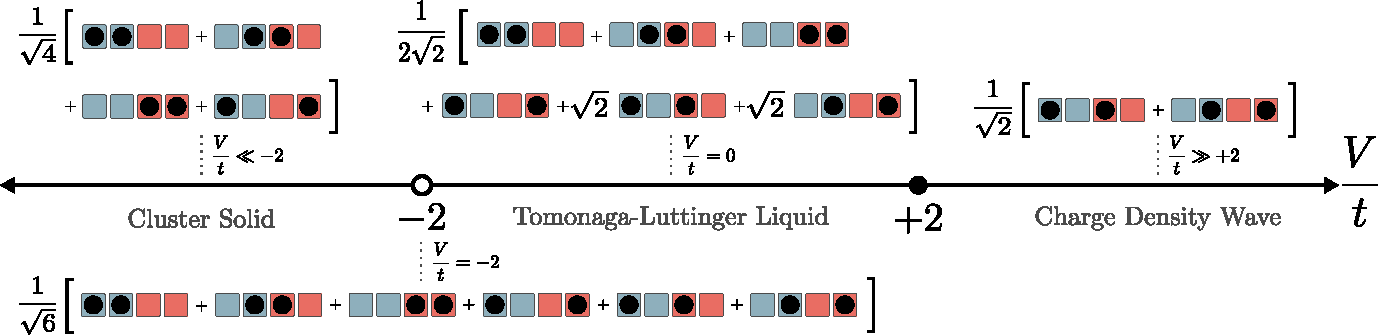
\includegraphics[width=1.0\textwidth]{phaseDiagramTV.pdf}
\end{center}
\caption{Phase diagram of the $t-V$ model accompanied by pictures of candidate ground states for $N=2$ fermions on a $L=4$ site lattice. For the purposes of measuring accessible entanglement, the lattice has been bipartitioned into spatial subregions $A$ (blue) and $B$ (red), each of size $\ell = 2$. We assume periodic boundary conditions. In the limit of strong attractive interactions where $V/t \ll -2$, the particles cluster together and there are $L$ equally probable configurations corresponding to all translations of the cluster.  At the first order phase transition where $V/t = -2$, all ${L}\choose{N}$ configurations are equally probable resulting in a flat state. In the TLL phase with $|V/t| < 2$,  particles are delocalized and we have included a characteristic state corresponding to free fermions $(V=0)$. In the limit of strong repulsive interactions where $V/t \gg 2$, fermions maximize their distance from each other resulting in a charge density wave (CDW) phase. The open and closed circles on the $V/t$ axis denote a first order and continuous phase transition, respectively.}
\label{fig:phaseDiagram}
\end{figure*}
%%%%%%%%%%%%%%%%%
\fi

\section{Numerical Results}


%In this section, numerical results obtained using exact diagonalization are shown. First, the finite size scaling of $S_{\alpha}^{\rm acc}(\rho_{A})$ will be illustrated. Following, the results correp

\subsection{Finite size scaling of the accessible entanglement}


%
%%%%%%%%%%
\begin{figure}[h!]
\begin{center}
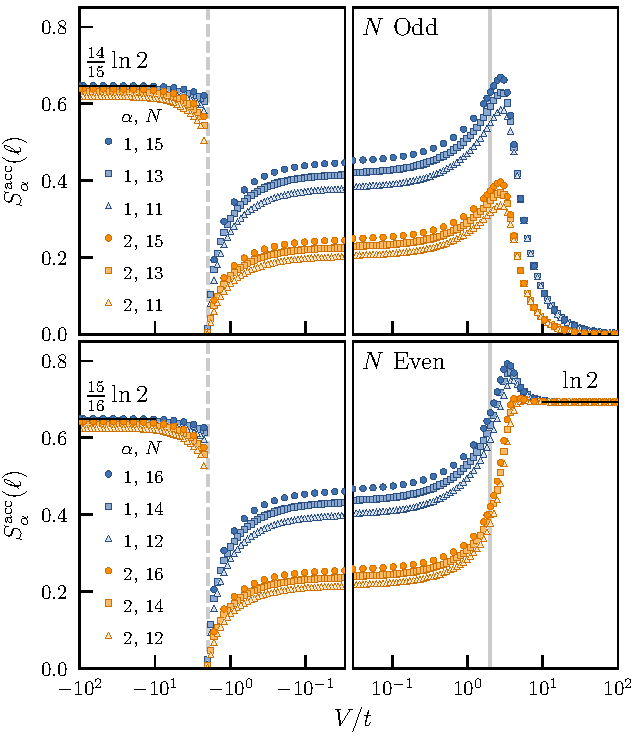
\includegraphics[scale=1.0]{operationalEntanglementEntropies_SOP5.pdf}
\end{center}
\caption{Accessible entanglement entropy $S_{\alpha}^{\mathrm{acc}}(\ell)$ for $\alpha = 1, 2$ in the ground state of the $t-V$ model as a function of interaction strength $V/t$. The top panel shows the results for an odd number of total particles: $N=11,13,15$ and the bottom, for even: $N=12,14,16$. The gray vertical lines indicate the locations of the known phase transitions for the model, $V/t = \pm 2$. For $N=15,16$ the asymptotic results computed in Section~\ref{tab:Limits} in the limits $V/t \to \pm \infty$ for $S_{1}^{\mathrm{acc}}$ are shown.}
\label{fig:OEE}
 \end{figure}
%%%%%%%%%%

Figure \ref{fig:OEE} shows the accessible R\'enyi entanglement entropy values at interaction strengths in the interval $V/t: \left( -100,100 \right)$. This interval spans the three phases of the $t-V$ model. For large negative interaction strengths, there is agreement between the values at which $S_{\alpha}^{\rm acc}(\rho_A)$ converges and the predicted value from \ref{tab:Limits} for all system sizes and $\alpha$. For large positive interaction strengths, the predicted effect of total particle number parity is observed. For $N$ odd, the accessible entanglement vanishes, whereas it converges to $\ln{2} \approx 0.6931 \dots$ for $N$ even, independent of system size and $\alpha$. At the first order phase transition $V/t=-2$, $S_{\alpha}^{\rm acc}(\rho_A)$, as expected. Thus, the asymptotic predictions for the accessible entanglement entropy in the $t-V$ model have been confirmed via exact diagonalization. Increasing the magnitude of both the attractive and repulsive interactions will result in even more agreement between simulation and theory.

Recall that the accessible entanglement should be a monotonically decreasing function of $\alpha$. Figure $\ref{fig:OEE}$ supports this inverse relation since it is seen that $S_{1} \geq S_{2}$ $\forall$ $V/t \in \left( -100,100 \right)$.

Another interesting feature is the peak seen near the continuous phase transition $V/t=2$. Results seem to indicate that the peak is slightly shifting to the left, closer to $V/t=2$ as the number of particles $N$ increases. In an effort to find how the location of this peak scales with particle number, $V/t\vert_{Max}$ was obtained for various system sizes, where $V/t\vert_{Max}$ is the interaction strength at which the accessible entanglement peak occurs. Figure \ref{fig:peakScalingOddN} shows a plot of $V/t\vert_{Max}$ vs $N^{-0.2545}$. The exponent comes from a linear fitting of $\left( V/t\vert_{Max} - 2 \right)$ vs $N$ data. The observed inverse power law scaling is promising as all points fall on a line with $y$ intercept of $V/t\vert_{Max} = 2$, which is the exact value of the continuous phase transition in the asymptotic limit of $N \to \infty$ total particles. Nevertheless, most of the system sizes in the data fall roughly in the same order of magnitude. The exact value of the phase transition $V/t = 2$ is obtained in the thermodynamic limit of $N\to\infty$ particles. Thus, to confirm the veracity of a power-law scaling of the peak of entanglement, more data points will be needed. Deviations from the line are noticeable in the largest three points presented. This suggests that there might be sub-leading terms that will hopefully become negligible for large system sizes. Currently, data for larger system sizes is being generated via Density Matrix Renormalization Group (DMRG) that will allow for the simulation of $N\approx100$ fermions \cite{SCHOLLWOCK201196} .

%%%%%%%%%%
\begin{figure}[h!]
\begin{center}
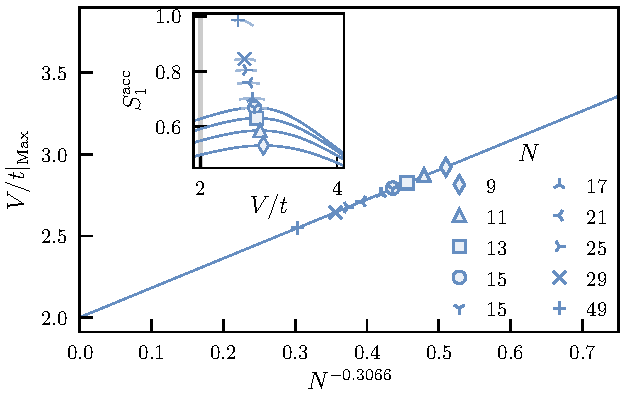
\includegraphics[scale=1.25]{peakScalingOddN.pdf}
\end{center}
\caption{Interaction strength at which the maximum $S_{1}^{\mathrm{acc}}$ occurs as a function of the total number of particles $N$. The exponent of $N$ was obtained from a linear fitting of $\ln N$ vs. $\ln{(V/t - 2)}$.  Although very few points are plotted due to memory limitations, they agree with the hypothesis that for $N \to \infty$, the peak of von Neumann accessible entanglement occurs at the phase transition $V/t = 2$. Inset: $S_{1}^{\mathrm{acc}}$ as a function of interaction strength $V/t$ for various $N$ around the neighborhood of the peak.}
\label{fig:peakScalingOddN}
\end{figure}
%%%%%%%%%%

\subsection{Entanglement of local particle number fluctuations}

Recall from section \ref{sec:accEntanglementIntro} that the difference between the full and the operationally accessible von Neumann entropies $\left( \alpha = 1 \right)$ should equal the Shannon entropy of the local particle number probability distribution $P_n$:
%
\begin{equation}
    \Delta S_1 (\rho_A) \equiv S_1(\rho_A) - S_1^{\rm acc}(\rho_A) = H_1(\{P_n\})
    \label{eq:DeltaS1}
\end{equation}
%
where
%
\begin{equation}
    H_1(\{P_n\}) = -\sum_{n=0}^N P_n \ln P_n.
\label{eq:H1}
\end{equation}
%
is the Shannon entropy of the probability distribution of the local particle number $P_n$.

In this section, a comparison is done between the Shannon entropy of the local particle number distribution and the difference between full and accessible entanglement. First, numerical results for this difference will be shown for the case of $\alpha=1$ and compared to the exact value of the Shannon entropy of normally distributed local particle numbers. Then, higher values of $\alpha$ will be studied and the difference will be compared with the Shannon entropy of the corresponding probability distribution of local particle number.

 %%%%%%%%%%
\begin{figure}[h!]
\begin{center}
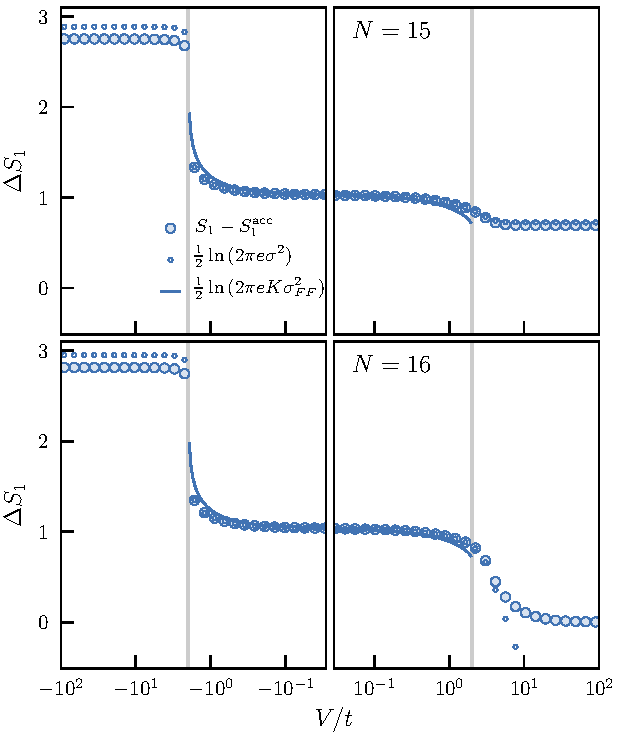
\includegraphics[scale=1.0]{deltaS1_N15N16.pdf}
\end{center}
\caption{Difference between the von Neumann and accessible entanglement entropies $S_{1}-S_{1}^{acc}$ and $\frac{1}{2} \ln 2 \pi e \sigma^2$ as functions of interaction strength $V/t$. The latter expression is the well known differential entropy of a Gaussian distribution. In TLL phase ($-2 < V/t < 2$), the probability distribution is Gaussian, as can be seen from the agreement between the two results. The solid lines use the theoretical variance of particle number in $A$ inside the $LL$ phase, $K \sigma^2_{FF}$, where $K$ is the Luttinger parameter and is a function of $V/t$ and $\sigma^2_{FF}$ is the exact variance for free-fermions ($V/t = 0$).}
\label{fig:deltaS1}
\end{figure}
%%%%%%%%%%

%
Figure \ref{fig:deltaS1} shows the difference between the full and accessible von Neumann entanglement entropies as a function of interaction strength. From exact diagonalization, the full ($S_1$), accessible ($S_{1}^{\rm acc}$) von Neumann entanglement entropies and the variance of local particle number $n$ ($\sigma$) were obtained. Expecting that local particle number fluctuations are normally distributed in the TLL phase ($-2 < V/t < 2$) of the $t-V$ model, these variances were inserted into the expression for the Shannon entropy of a Normal Distribution $\frac{1}{2}\ln{\left( 2\pi e \sigma^2 \right)}$. Additionally, the Shannon entropy was calculated using the variance of local particle number predicted by Tomonaga-Luttinger Liquid theory $\sigma \equiv K\sigma_{FF}$ where $\sigma_{FF}$ is the variance of free-fermions $V/t = 0$ and $K$ is the Luttinger Parameter $K = \pi/(\cos^{-1}\left( -V/2t \right))$, as shown in Chapter 2 . The figure shows agreement between the three expressions in the TLL phase.


%%%%%%%%%%
\begin{figure}[h!]
\begin{center}
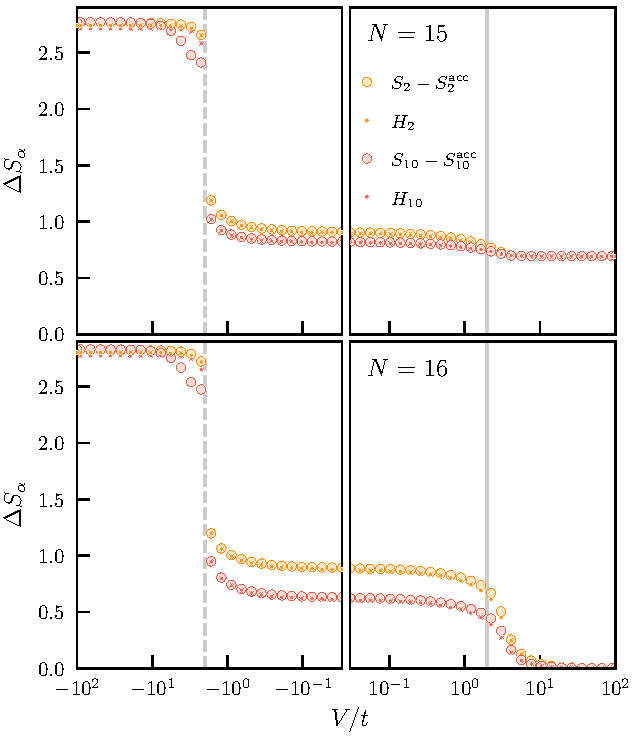
\includegraphics[scale=1.0]{higherAlphaDeltaS_N15N16.pdf}
\end{center}
\caption{Difference between the \ren and accessible entanglement entropy $S_{\alpha} - S_{\alpha}^{\mathrm{acc}}$ and $H_{\alpha}$ as functions of interaction strength $V/t$ for $\alpha=2,10$. In general, $H_{\alpha}$ should provide a lower bound for $\Delta S_{\alpha}$ (i.e, $H_{\alpha} \leq S_{\alpha}$). Also, $S_{\alpha}^{\mathrm{acc}}$ should be non-increasing in $\alpha$. It can be seen that both relations hold in all phases of the $t-V$ model.}
\label{fig:deltaS_alpha}
\end{figure}
%%%%%%%%%%

At R\'enyi indices higher than $\alpha = 1$, the difference between the full and accessible entanglement entropies should be bounded from below by the classical R\'enyi entropy of the local particle number probability distribution $H_{\alpha}\left(\{P_n\}\right) = \ln{ \sum_{n} P_{n}^{\alpha}}/(1-\alpha)$. Figure \ref{fig:deltaS_alpha} shows $\Delta S_{\alpha}$ and $H_{\alpha}\left(\{P_n\}\right)$ as a function of interaction strength for R\'enyi indices $\alpha=2$ and $\alpha=10$. Not only in all cases is $H_{\alpha}\left(\{P_n\}\right) \leq \Delta S_{\alpha}$, but also the values corresponding to $\alpha=10$ are lower than the ones corresponding to $\alpha=2$, satisfying the condition that the difference in full and accessible entanglement should be a monotonically decreasing function of $\alpha$. The fact there's such good agreement for the $\alpha=2$ and $\alpha=10$ is rather astounding. Taking a look at Figure $\ref{fig:Halpha}$ reveals that the difference between the computationally determined R\'enyi entropy of $P_n$ and the theoretical value is proportional to the R\'enyi index. For $\alpha=10$, this difference is large enough that the agreement in the TLL phase in Figure \ref{fig:deltaS_alpha} is surprising. Up next, it will be shown that this agreement is a result of the proportionality between $P_{n,\alpha}$ and $P_n^{\alpha}$.

%%%%%%%%%%
\begin{figure}[h!]
\begin{center}
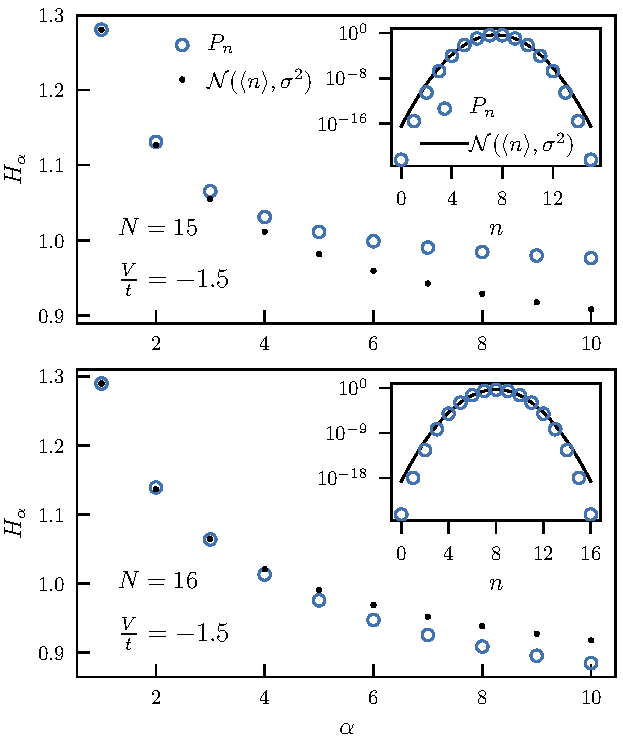
\includegraphics[scale=1.0]{Halpha.pdf}
\end{center}
\caption{For $N=15$, $\sigma^2=0.758$ and for $N=16$, $\sigma^2=0.772$.}
\label{fig:Halpha}
 \end{figure}
%%%%%%%%%%

Recall the distribution defined in section \ref{sec:accEntanglementIntro}:
%
\begin{equation}
P_{n,\alpha} = \frac{P_{n}}{\Tr\rho_{A}^{\alpha}}
\label{eq:Pna}
\end{equation}
 %
 
which due to a normal distribution of local particle numbers  in the TLL phase of the $t-V$ model ($-2 < V/t < 2$) can be approximated as:
%
\begin{equation}
P_{n,\alpha} \approx \sqrt{\frac{\pi\alpha}{2K\ln{\ell}}} e^{\frac{-\alpha \pi^2 (n - \langle n \rangle^2 )}{2K\ln{\ell}}} 
\label{eq:Pna_TLL}
\end{equation}
 %
 
Notice that raising Eq.~\eqref{eq:Pna_TLL} to either $1/\alpha$ or $K$ on both sides should get rid of the $\alpha$ or $K$ dependence of the exponential factor, respectively, within the TLL regime. The square root factor will still pick up the dependence on either of the exponents. In other words, raising by $1/\alpha$ or $K$ should give:
 %
 \begin{equation}
 P_{n,\alpha}^{1/\alpha} \approx \sqrt{\frac{\pi\alpha}{2K\ln{\ell}}}^{1/\alpha} e^{\frac{- \pi^2 (n - \langle n \rangle^2 )}{2K\ln{\ell}}} 
 \label{eq:Pna_to_alphaInv}
 \end{equation}
 %
 and
 %
 \begin{equation}
 P_{n,\alpha}^{K} \approx \sqrt{\frac{\pi\alpha}{2K\ln{\ell}}}^K e^{\frac{- \alpha \pi^2 (n - \langle n \rangle^2 )}{2\ln{\ell}}} 
 \label{eq:Pna_to_K}
 \end{equation}
 %
 %%%%%%%%%%
\begin{figure}[h!]
\begin{center}
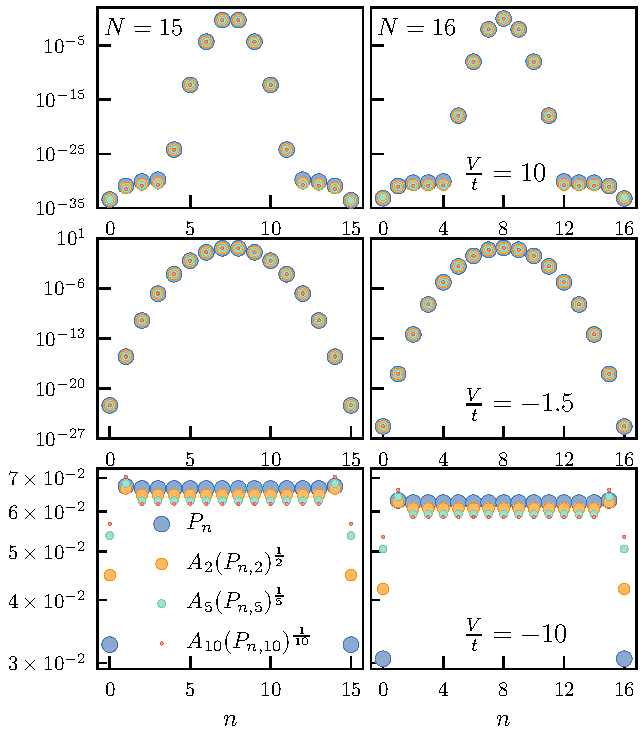
\includegraphics[scale=1.1]{alphaCollapse.pdf}
\end{center}
\caption{Probabilities of measuring a state with $n$ particles in subregion $A$, as  a function of $n$. The probabilities in the $TLL$ regime are known to be Gaussian. Here, they have been raised to $1/\alpha$ in order to cancel out the $\alpha$ dependence of the exponential part. For the middle plot, the interaction strength lies in the $TLL$ regime and, consequently, the probabilities collapse to the same values in all the range after the $\alpha$ dependence has been cancelled. The top and bottom plots show results outside of the $TLL$ regime, where the probabilities are not Gaussian.}
\label{fig:alpha_collapse}
\end{figure}
%%%%%%%%%%
 
 Figure \ref{fig:alpha_collapse} shows the distribution $A_{\alpha} P_{n,\alpha}^{1/\alpha}$ for various interaction strengths $V/t$ and, thus, $K$. The constant $A_{\alpha}$ is the inverse of the square root factor in Eq.~\eqref{eq:Pna_to_alphaInv}. Cancelling the square root factor allows for a direct comparison of the exponential factor for each of the $\alpha$ values used. The middle plots confirm that this exponential factor indeed is independent of $\alpha$, illustrated by the fact that the distributions become the same for $\alpha=\{1,2,5,10\}$, when inside the TLL regime of $-2 < V/t < 2$.
 
%%%%%%%%%%
\begin{figure}[h!]
\begin{center}
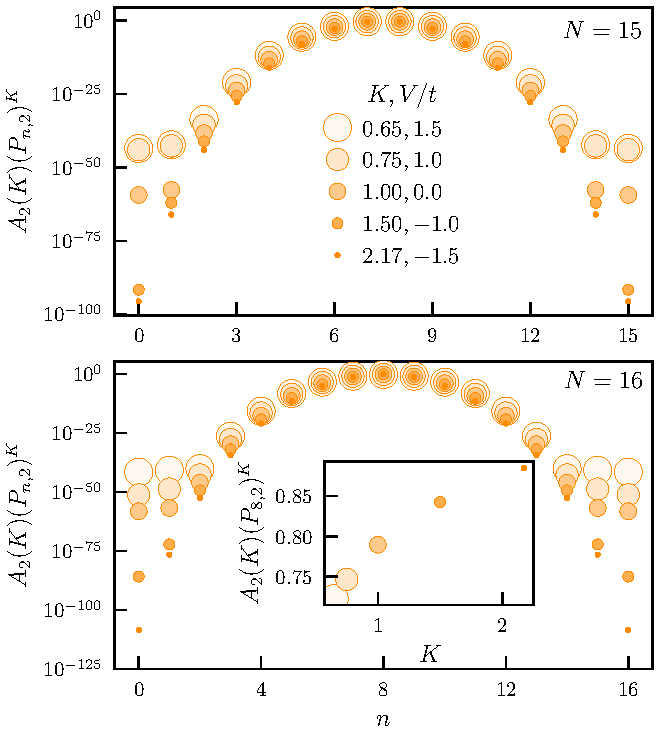
\includegraphics[scale=1.0]{TLLCollapse.pdf}
\end{center}
\caption{Probabilities of measuring a state with $n$ particles in subregion $A$, as  a function of $n$. This time, the probabilities have been raised to the Luttinger Parameter $K$, after calculating for several $K$ values. The probabilities seem to collapse nearly to the same value near the middle of the distribution. The inset plot shows the $K$ dependence of the probability for fixed particle number in $A$, $n=8$. This helps illustrate that the probabilities are proportional to $K$ near the middle, as opposed to inversely proportional at the ends.}
\label{fig:K_collapse}
\end{figure}
%%%%%%%%%%
 
Figure \ref{fig:K_collapse} shows the distribution $A_{\alpha} P_{n,\alpha}^{K}$ with the R\'enyi index fixed at $\alpha=2$ and at various interaction strengths $V/t$ and corresponding Luttinger parameters $K$. In this case, the factor $A_{\alpha}$ is the inverse of the square root factor in Eq.~\eqref{eq:Pna_to_K}. All of the interaction strengths fall within the TLL regime and as such, all the distributions should become the same for the various $V/t$ and, thus, $K$ values. This collapse of the distributions at various $K$ is evident from looking at regions near the middle of the graph. Although it may not be apparent at first glance due to the scale, the tails of the distribution are all essentially zero.

\section{Conclusion}
In this chapter, the operationally accessible R\'enyi entanglement entropy was introduced in both it's original and generalized form. Analytical values of the entanglement entropy were obtained at various special cases of the $t-V$ model and then confirmed via exact diagonalization. A maximum value in accessible entanglement was observed and evidence seems to support that it follows an inverse power law scaling in total particle number with scaling exponent -0.2545. 

The difference in full and accessible entanglement entropies was also computationally determined and it was confirmed that in the TLL phase of the $t-V$ model, it is equal to the the R\'enyi entropy of a Normal Distribution of local particle number. Finally, it was then proposed theoretically and confirmed computationally, that getting rid of its R\'enyi index and Luttinger parameter dependence, the exponential part of these Normal Distributions depend exclusively on local particle number fluctuations.


